\chapter{Résultats de simulation}
\label{ch:simulation}

\section{Testbench}

Le testbench (\ref{testbench}) génère une horloge et un signal de
réinitialisation actif pendant les premiers cycles d'horloge.

\lstinputlisting[language=VHDL, caption=\texttt{testbench.vhd}, label=testbench,
    basicstyle=\ttfamily\footnotesize]{../vhdl/testbench.vhd}

\section{Test du processeur}

Pour tester le processeur, on peut s'assurer que l'exécution de certains
programmes donne bien les résultats attendus : après avoir simulé le
fonctionnement du processeur à l'aide du testbench, on étudie les valeurs de
certains signaux et registres d'intérêt. \\

\begin{figure}[h]
    \centering
    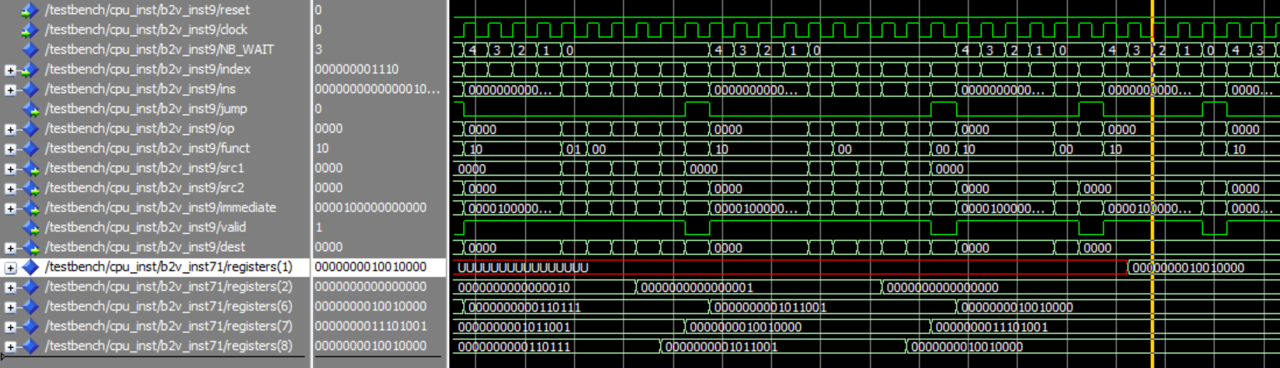
\includegraphics[width=\textwidth]{figures/simulation.png}
    \caption{Résultats de la simulation avec \texttt{fibo.out}}
    \label{fig:simulation}
\end{figure}

Avec le programme \texttt{fibo.out} (résultats en figure \ref{fig:simulation}),
l'évolution de \texttt{NB\_WAIT}, \texttt{index} et \texttt{ins} semble
confirmer la bonne gestion des sauts. De plus, la valeur finale stockée dans
\texttt{x1} est $0b10010000 = 144$. Or $F_{12} = 144$: on a bien le résultat
attendu ! \\

En revanche, cela ne prouve pas le bon fonctionnement du processeur, car
l'ensemble de ses fonctionnalités n'est pas exhaustivement testé par
\texttt{fibo.asb}. En particulier, la pile n'est pas utilisée.
